\documentclass[a4paper]{article}

\usepackage[english]{babel}
\usepackage[utf8]{inputenc}
%\usepackage[OT4]{fontenc}
\usepackage{amsmath}
\usepackage{graphicx}
\usepackage[colorinlistoftodos]{todonotes}
\usepackage{geometry}
\usepackage{titlesec}
\usepackage{multirow}
\usepackage[autostyle]{csquotes}
\usepackage[backend=biber,style=numeric]{biblatex}

\addbibresource{discrete-petri.bib}

\geometry{
	a4paper,
    left=1in,
    right=1in,
    top=1.5in,
    bottom=1.5in
}

\renewcommand{\familydefault}{\sfdefault}
\renewcommand{\baselinestretch}{1.75}

\providecommand{\e}[1]{\ensuremath{\times 10^{#1}}}

\setlength{\parindent}{2em}

\titlespacing*{\section} {0pt}{0.3in}{0.3in}
\titlespacing*{\subsection} {0pt}{0.3in}{0.3in}

\title{Petri Networks\\Modeling, simulation, and performance analysis of discrete event systems used in electrical engineering}

\author{\\Authors:\\ Kamil Jamroz,\\ Michal Raton,\\ Adam Zelazowski\\}

\date{\today}

\begin{document}

\nocite{*}

\maketitle

\clearpage

\tableofcontents

\clearpage

% -------------------------------------------------------------
%
\section{Foreword}
\label{cha:foreword}
\paragraph{}

For our project in "Modeling, simulation, and performance analysis of discrete event systems with Petri-Nets", we have chosen to simulate a part of power grid used in Poland. Our statistical analysis takes into account both physical properties of cables and real topology on which power grid bases on. The reason for choosing this project is the fact that we believe Petri-nets are perfect tools for simulation such scenario, and we would like to evaluate if this statement will hold true throughout the project. This report will be divided in several parts and cover input data, simulation files, diagrams and received results.

% -------------------------------------------------------------
%
\section{Introduction}  
\label{cha:introduction}
\paragraph{}

Rising consumption of electrical energy and its strategic meaning in economy of highly developed countries has translated into creation of necessity to guarantee safety of its supply to customers. The fundamental limitations regarding the capacity of modern electrical networks are set because of physical properties of materials used in their construction. Each material has its own set of properties and cost of use, both of which have to be taken into consideration by electrical engineers in phase of designing new and maintaining existing power grid connections. For the purpose of current document we had chosen a part of the power grid existing in Poland and simulated what would happen if links between parts of the grid were overloaded - where would the power go and how would it affect the state of the network. Specifically, we tried to simulate how much would cables extend if more power were transmitted through them and checked whether there exists possibilities of accidents.

\subsection{Problem definition}
\label{sec:problemDefinition}
\paragraph{}

The biggest problem connected to creation of new and maintaining existing power grids is the fact that depending on the load in the given unit of time the physical reaction of power grid infrastructure can be different. The voltage transported through the cables make huge impact on them changing their characteristics such as length, temperature and others. What's more they are also dependent on external factors - the time of the day, the season, air temperature etc. The plethora of scenarios that must be taken into consideration makes fixing power grids hard and expensive.

\subsection{Goals} 
\label{sec:goals}
\paragraph{}

The are few goals of this project. The first one is to check whether Petri-nets are well-fit tool for purpose of modeling and evaluating electrical networks. We will decide on this depending on the results we get from simulating existing power grid. The second one is to validate existing power grid topology, check whether it is optimal and efficient or has the used topology started to show its age. 

\subsection{Sources}
\label{sec:sources}
\paragraph{}
The sources used in this project are the topology of Polish power grid with its physical properties, average power consumption data scaled up to appropriate values. The theory we used for the purpose of this document was taken from our our understanding of basics of physics and electrical engineering, science magazines and information we gained while searching internet for suitable articles on this matter.

\subsection{Methods}
\label{sec:methods}
\paragraph{}

As a tool for modeling and simulation the existing power grid we will use Petri-nets. The places will represent customers while transitions will represent cables. The markers will be used as a mean of representing electrical movement. The tool we will use for this project is GPenSIM created by Reggie Davidrajuh \cite{Art2}. The details of used method will be described further in its own section.

\clearpage

% -------------------------------------------------------------
%
\section{Theory}
\label{cha:theory}
\paragraph{}

In this section we will try to describe basic concepts that needs to be known by the reader to properly understand this document.

\subsection{Petri networks}
\label{sec:petriNetworks}
\paragraph{}

\textbf{Petri networks} (Petri-nets) is one of several mathematical modeling languages for the description of distributed systems. A Petri net is a directed bipartite graph, in which the nodes represent transitions (i.e. events that may occur, represented by bars) and places (i.e. conditions, represented by circles). The directed arcs describe which places are pre- and/or post- conditions marked  as arrows. \cite{Art3}

In mathematical sense Petri-net can be described as a tuple:

\begin{equation}
N = ( P, T, A, N, E, G, I )
\end{equation}

where:
\begin{itemize}
	\setlength{\itemsep}{1pt}
	\setlength{\parskip}{0pt}
	\setlength{\parsep}{0pt}
\item P is a set of places,
\item T is a set of transitions,
\item A is a set of arcs,
\item N is a node function. It maps A into (P $\times$ T) $\bigcup$ (T $\times$ P),
\item E is an arc expression function. It maps each arc into the expression e. The input and output types of the arc expressions must correspond to the type of the nodes the arc is connected to,
\item G is a guard function. It maps each transition into guard expression g. The output of the guard expression should evaluate to Boolean value true or false,
\item I is an initialization function. It maps each place p into an initialization expression i. The initialization expression must evaluate to multiset of tokens with a color corresponding to the color of the place C(p).\\
\end{itemize}

\clearpage

An extension of Petri-nets are \textbf{Coloured Petri-nets}. They allow tokens to have a data value attached to them. This attached data value is called token color. Although the color can be of arbitrarily complex type, places usually contain tokens of one type. This type is called color set of the place. \cite{Art4} Color sets can be compared to structures in prototype programming.\\

The second extension of Petri-nets used are \textbf{Prioritized Petri-nets}. They allow to solve conflicts in queuing firing the transitions thanks to using priorities. In case of conflict between two or more transitions the one with higher priority wins.

\subsection{Thermodynamics}
\label{sec:thermodynamics}
\paragraph{}

For the purpose of this project we had to use basic information from physics. The main concepts we had to use are fundamentals of thermodynamics.\\

\textbf{Thermodynamics} is a branch of physics concerned with heat and temperature and their relation to energy and work. It defines macroscopic variables, such as internal energy, entropy, and pressure, that partly describe a body of matter or radiation. \cite{Art5}\\

One of sub occurrences of this subject of physics is \textbf{Thermal expansion}. It defines the tendency of matter to change in shape, area, and volume in response to a change in temperature, through heat transfer. The coefficient of thermal expansion describes how the size of an object changes with a change in temperature. Specifically, it measures the fractional change in size per degree change in temperature at a constant pressure. \cite{Art1}\\

To measure the value of extension or contraction of the length for given material, the following formula can be used: \cite{Art6}

\clearpage

\begin{equation}
x = x_{0} (1 + \alpha \Delta T)
\end{equation}

where:
\begin{itemize}
	\setlength{\itemsep}{1pt}
	\setlength{\parskip}{0pt}
	\setlength{\parsep}{0pt}
\item $x$ is the length of material after expansion,
\item $x_{0}$ is the length at the start of the process,
\item $\alpha$ is thermal expansion coefficient,
\item $\Delta T$ is the relative change of temperature.\\
\end{itemize}

To value of thermal expansion coefficient is defined as: 

\begin{equation}
\alpha = \frac {x - x_{0}} {x_{0} \Delta T} = \frac {\Delta x} {x_{0} \Delta T}
\end{equation}

Where the unit is:

\begin{equation}
[\alpha] = \frac {1}{K}
\end{equation}

The relative change of temperature can be found using equation: \cite{Art7}

\begin{equation}
R_T=R_0(1+\alpha \cdot \Delta T)
\end{equation}

where:
\begin{itemize}
	\setlength{\itemsep}{1pt}
	\setlength{\parskip}{0pt}
	\setlength{\parsep}{0pt}
\item $R_T$ is resistance for temperature $T$,
\item $R_0$ is resistance for temperature $T_0$,
\item $\alpha$ is thermal resistance coefficient,
\item $\Delta T$ is the relative change of temperature.\\
\end{itemize}

The thermal resistance coefficient depends on the material for which we are making calculations. In our project we focus on electrical ALF wires which are made of aluminium, so we can assume:

\begin{equation}
\alpha = 2.4\e{-5} [K^{-1}]
\end{equation}

\subsection{Power transfer and power loss}
\label{sec:powerTransferAndPowerLoss}
\paragraph{}

The second concept that needs to be understand to properly simulate powergrid is the \textbf{energy loss}.\\ 

Transmitting electricity at high voltage reduces the fraction of energy lost to resistance, which varies depending on the specific conductors, the current flowing, and the length of the transmission line. Factors that affect the resistance, and thus loss, of conductors used in transmission and distribution lines include temperature, spiraling, and the skin effect. The resistance of a conductor increases with its temperature. Temperature changes in electric power lines can have a significant effect on power losses in the line. Spiraling, which refers to the increase in conductor resistance due to the way stranded conductors spiral about the center, also contributes to increases in conductor resistance. The skin effect causes the effective resistance of a conductor to increase at higher alternating current frequencies. \cite{Art8}\\

The power loss can be measured with:

\begin{equation}
\Delta P_0 = 3I^{2}R = 3\left(\frac {S}{\sqrt{3}U}\right) R = \frac {S^{2}}{U^{2}} R = \frac {P^{2} + Q^{2}}{U^{2}} R
\end{equation}

where:
\begin{itemize}
	\setlength{\itemsep}{1pt}
	\setlength{\parskip}{0pt}
	\setlength{\parsep}{0pt}
\item I is electrical current in conductor (9),
\item S, P, Q are, successively, apparent, true and reactive powers (8),
\item R is electrical resistance,
\item U is voltage.
\end{itemize}

The additional formulas used were:

\begin{equation}
P = \sqrt{3}UI\cos{\phi}
\end{equation}

\begin{equation}
I = \frac {P}{\sqrt{3}U\cos{\phi}}
\end{equation}

\clearpage

% -------------------------------------------------------------
%
\section{Methods}
\label{cha:methods}
\paragraph{}
Considering the low amount of time dedicated to the project and relative little experience in chosen subject, we limited the analysis to two properties -- thermal expansion and energy loss -- while transporting power through power lines. All calculations were made using formulas put in chapter \ref{cha:theory}, the properties of ALF power lines and external factors.

\subsection{Assumptions}
\label{sec:assumptions}
\paragraph{}

The simulated power grid consist of AFL-6 120, 185  and 240 power lines showed in figure \ref{fig:img1}. Their properties have been put in table \ref{tab:aflProperties}.

\begin{table}[!h]
\centering
\caption{Allowed long-term current {[}A{]}}
\label{tab:aflProperties}
\begin{tabular}{|l|l|l|l|l|l|l|}
\hline
\multicolumn{1}{|c|}{\multirow{3}{*}{Power line type}} & \multicolumn{6}{c|}{For lines designed for specific temperature}                     \\ \cline{2-7} 
\multicolumn{1}{|c|}{}                                & \multicolumn{2}{l|}{+40 C} & \multicolumn{2}{l|}{+60 C} & \multicolumn{2}{l|}{+80 C} \\ \cline{2-7} 
\multicolumn{1}{|c|}{}                                & Summer       & Winter      & Summer       & Winter      & Summer       & Winter      \\ \hline
AFL-6 120 mm                                          & 205          & 405         & 350          & 475         & 410          & 475         \\ \hline
AFL-6 185 mm                                          & 270          & 535         & 455          & 630         & 535          & 630         \\ \hline
AFL-6 240 mm                                          & 325          & 625         & 550          & 735         & 645          & 735         \\ \hline
\end{tabular}
\end{table}

\begin{figure}[h]
\centering
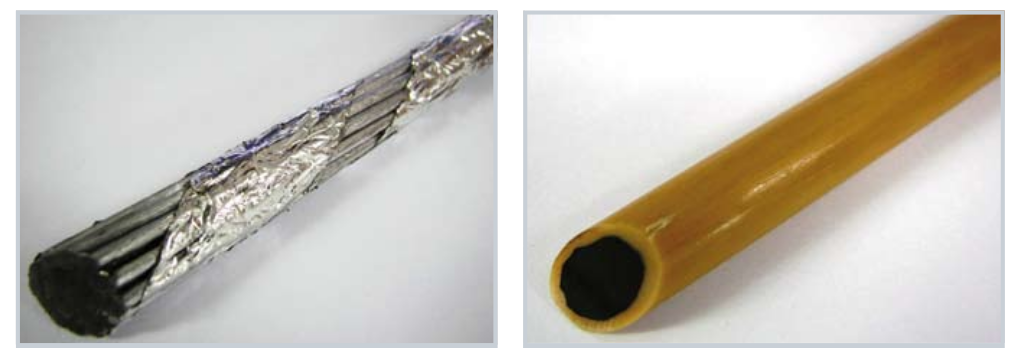
\includegraphics[scale=0.45]{schemas/img1.png}
\caption{\label{fig:img1}}
\end{figure}

\clearpage

The cross-section of typical AFL cable has been put in figure \ref{fig:img2}.

\begin{figure}[h]
\centering
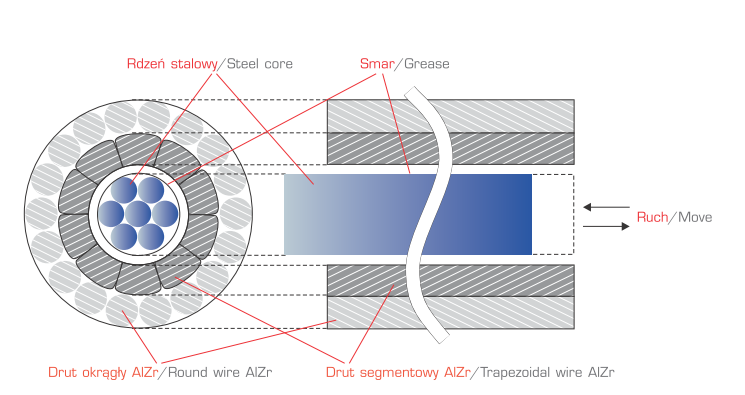
\includegraphics[scale=0.45]{schemas/img2.png}
\caption{\label{fig:img2}}
\end{figure}

Additionally, we had to make assumptions considering external factors that affects state of power grid, the variables and values used have been put in table \ref{tab:extProperties}. Most of them have been separately measured for two seasons -- Winter and Summer -- between which change in power grid state is the most apparent.\\

\begin{table}[!h]
\centering
\caption{External factors and values}
\label{tab:extProperties}
\begin{tabular}{|l|l|r|}
\hline
\multicolumn{1}{|c|}{Variable}    & \multicolumn{1}{c|}{Case} & \multicolumn{1}{c|}{Value} \\ \hline
\multirow{3}{*}{Line temperature} & AFL-6  120mm              & +40 C                      \\ \cline{2-3} 
                                  & AFL-6 185mm               & +60 C                      \\ \cline{2-3} 
                                  & AFL-6 240mm               & +80 C                      \\ \hline
\multirow{2}{*}{Air temperature}  & Summer                    & +30 C                      \\ \cline{2-3} 
                                  & Winter                    & -20 C                      \\ \hline
\multirow{2}{*}{Wind velocity}    & Summer                    & 0,5 m/s                    \\ \cline{2-3} 
                                  & Winter                    & 0,5 m/s                    \\ \hline
\multirow{2}{*}{Insolation}       & Summer                    & 1000 w/m2                  \\ \cline{2-3} 
                                  & Winter                    & 770 w/m2                   \\ \hline
Segment length                    & --                        & 185 m                      \\ \hline
\end{tabular}
\end{table}

\clearpage

% ze względu c na ograniczony wymiar godzin oraz relatywny brak doświadczenia w dziedzinie skupiliśmy się na aspekcie rozszerzalności tempereraturowej przewodów w zależności od obciążenia sieci, temperaratury zewnętrznej oraz typu przewodu biorąc pod uwagę temperaturowy współczynnik rezystancji materiału przewodzącego jakim jest aluminium w badanej sieci. W naszym modelu sieci zakładamy następujące założenia: 
% dwa przedziały temperatur zewnętrznych (lato +30 C , zima + 20 C)
% przedziały temperatur przeowodó  40/60/80 C
%- stała prędkość wiatru zgodna z wartościami z tabeli producenta (0,5 m/s) (prostopadle do przewodu)
% nasłonecznienie : lato 1000 W/m^2, zima 770 W/m^2    
% odległość między przęsłami w poszczególnych przewodach 185 metrów   

\subsection{Power grid}
\label{sec:powerGrid}
\paragraph{}

The power grid consists of three generators and N customers. We have modeled approximately realistic distances between them. Total length of all power lines is M. The topology has been shown in figure \ref{fig:img3}.\\\\

\begin{figure}[h]
\centering
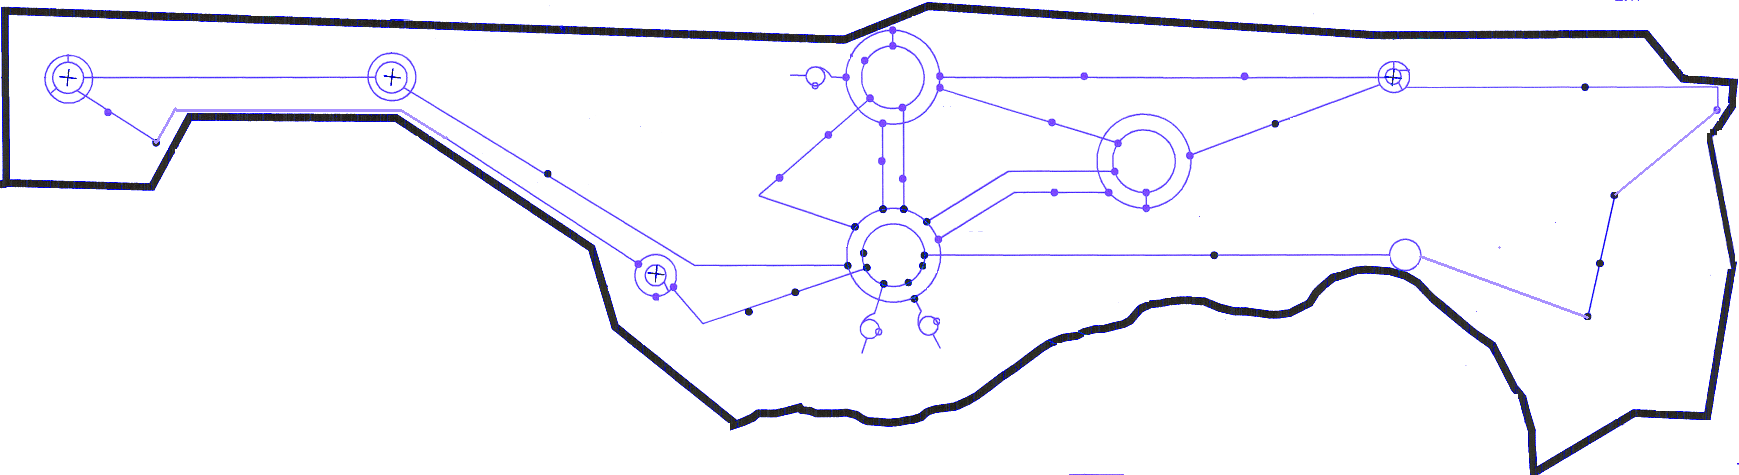
\includegraphics[scale=0.35]{schemas/img3.png}
\caption{\label{fig:img3}}
\end{figure}

Simulation has been divided into several sub-simulations of which each one represents only one power grid segment. This method allowed us to imitate the real way how the whole network works. The data about power usage and voltage has been approximated using statistical computing.

% symulacje przeprowadzamy badajc poszczegolne fragmenty sieci ze wzgledu an sposob w jaki w rzeczywistosci jest transmitowana energia. Dane o zuzyciu pradu i natezeniach niezbedne do przeprowadzenia symulacji sa rowniez przyblizonymi danymi statycznymi. 

\subsection{Petri-Net model}
\label{sec:petriNetModel}
\paragraph{}

The power grid showed in figure \ref{sec:powerGrid} has been translated to Petri-Net model. To design it properly we have used two extension of Petri-networks - colors and priorities.\\

%In our model we are using colored tokens and priorities. The colors 

The colored tokens is being used for representing the value of voltage transported through cables. In unit of time that marker enters each customer, the token value is being lowered by the amount of customer's power need, allowing program to effectively measure the energy loss. When it exceeds the starting value, then the whole marker is checked as used up and removed from the simulation. We would like to highlight the fact, that using colors enabled the simulation to be extended further for more electrical measurements.\\

% W naszym modelu sieci wykorzystujemy zarowno kolorowe tokeny i prirorytety. Kolory symoblizuja nad strate mocy na poszczegolnych odcinkach. Jezeli ilosc mocy spadnie do zera, to przerywamy symulacje, poniewz nie jest mozliwe zasilnenie kolejnego odbiorcy. Pragniemy zaznaczyc ze dzieki zastosowaniu kolorow mozna rozszerzyc symulacje o symulowanie innych wartosci zwiazanych z praca sieci. 

The priorities have been set to each power line and are used as routing mechanics to be able to choose how the power is transported to customers, specifically which segments are active. We have created a separate dynamic system in form of external function that allowed us to modify the flow of energy power during the simulation.\\

% priorytety sluza do wyboru segmentu sieci, ktory chcemy uwzglednic w symulacji. Dzieki nim wybor segmentu ogranciza sie do stworzenia tablciy z wezlami ktore uczestnicza w danej symulacji. Ponadt to dzieki funkcjom modyfikujacym priorytety mozna by przeprwozic symulacje uwzlegniajace dynamiczny przeplyw sieci.

The graphic representation of described model is shown in figure \ref{fig:img4}.\\

\begin{figure}[h]
\centering
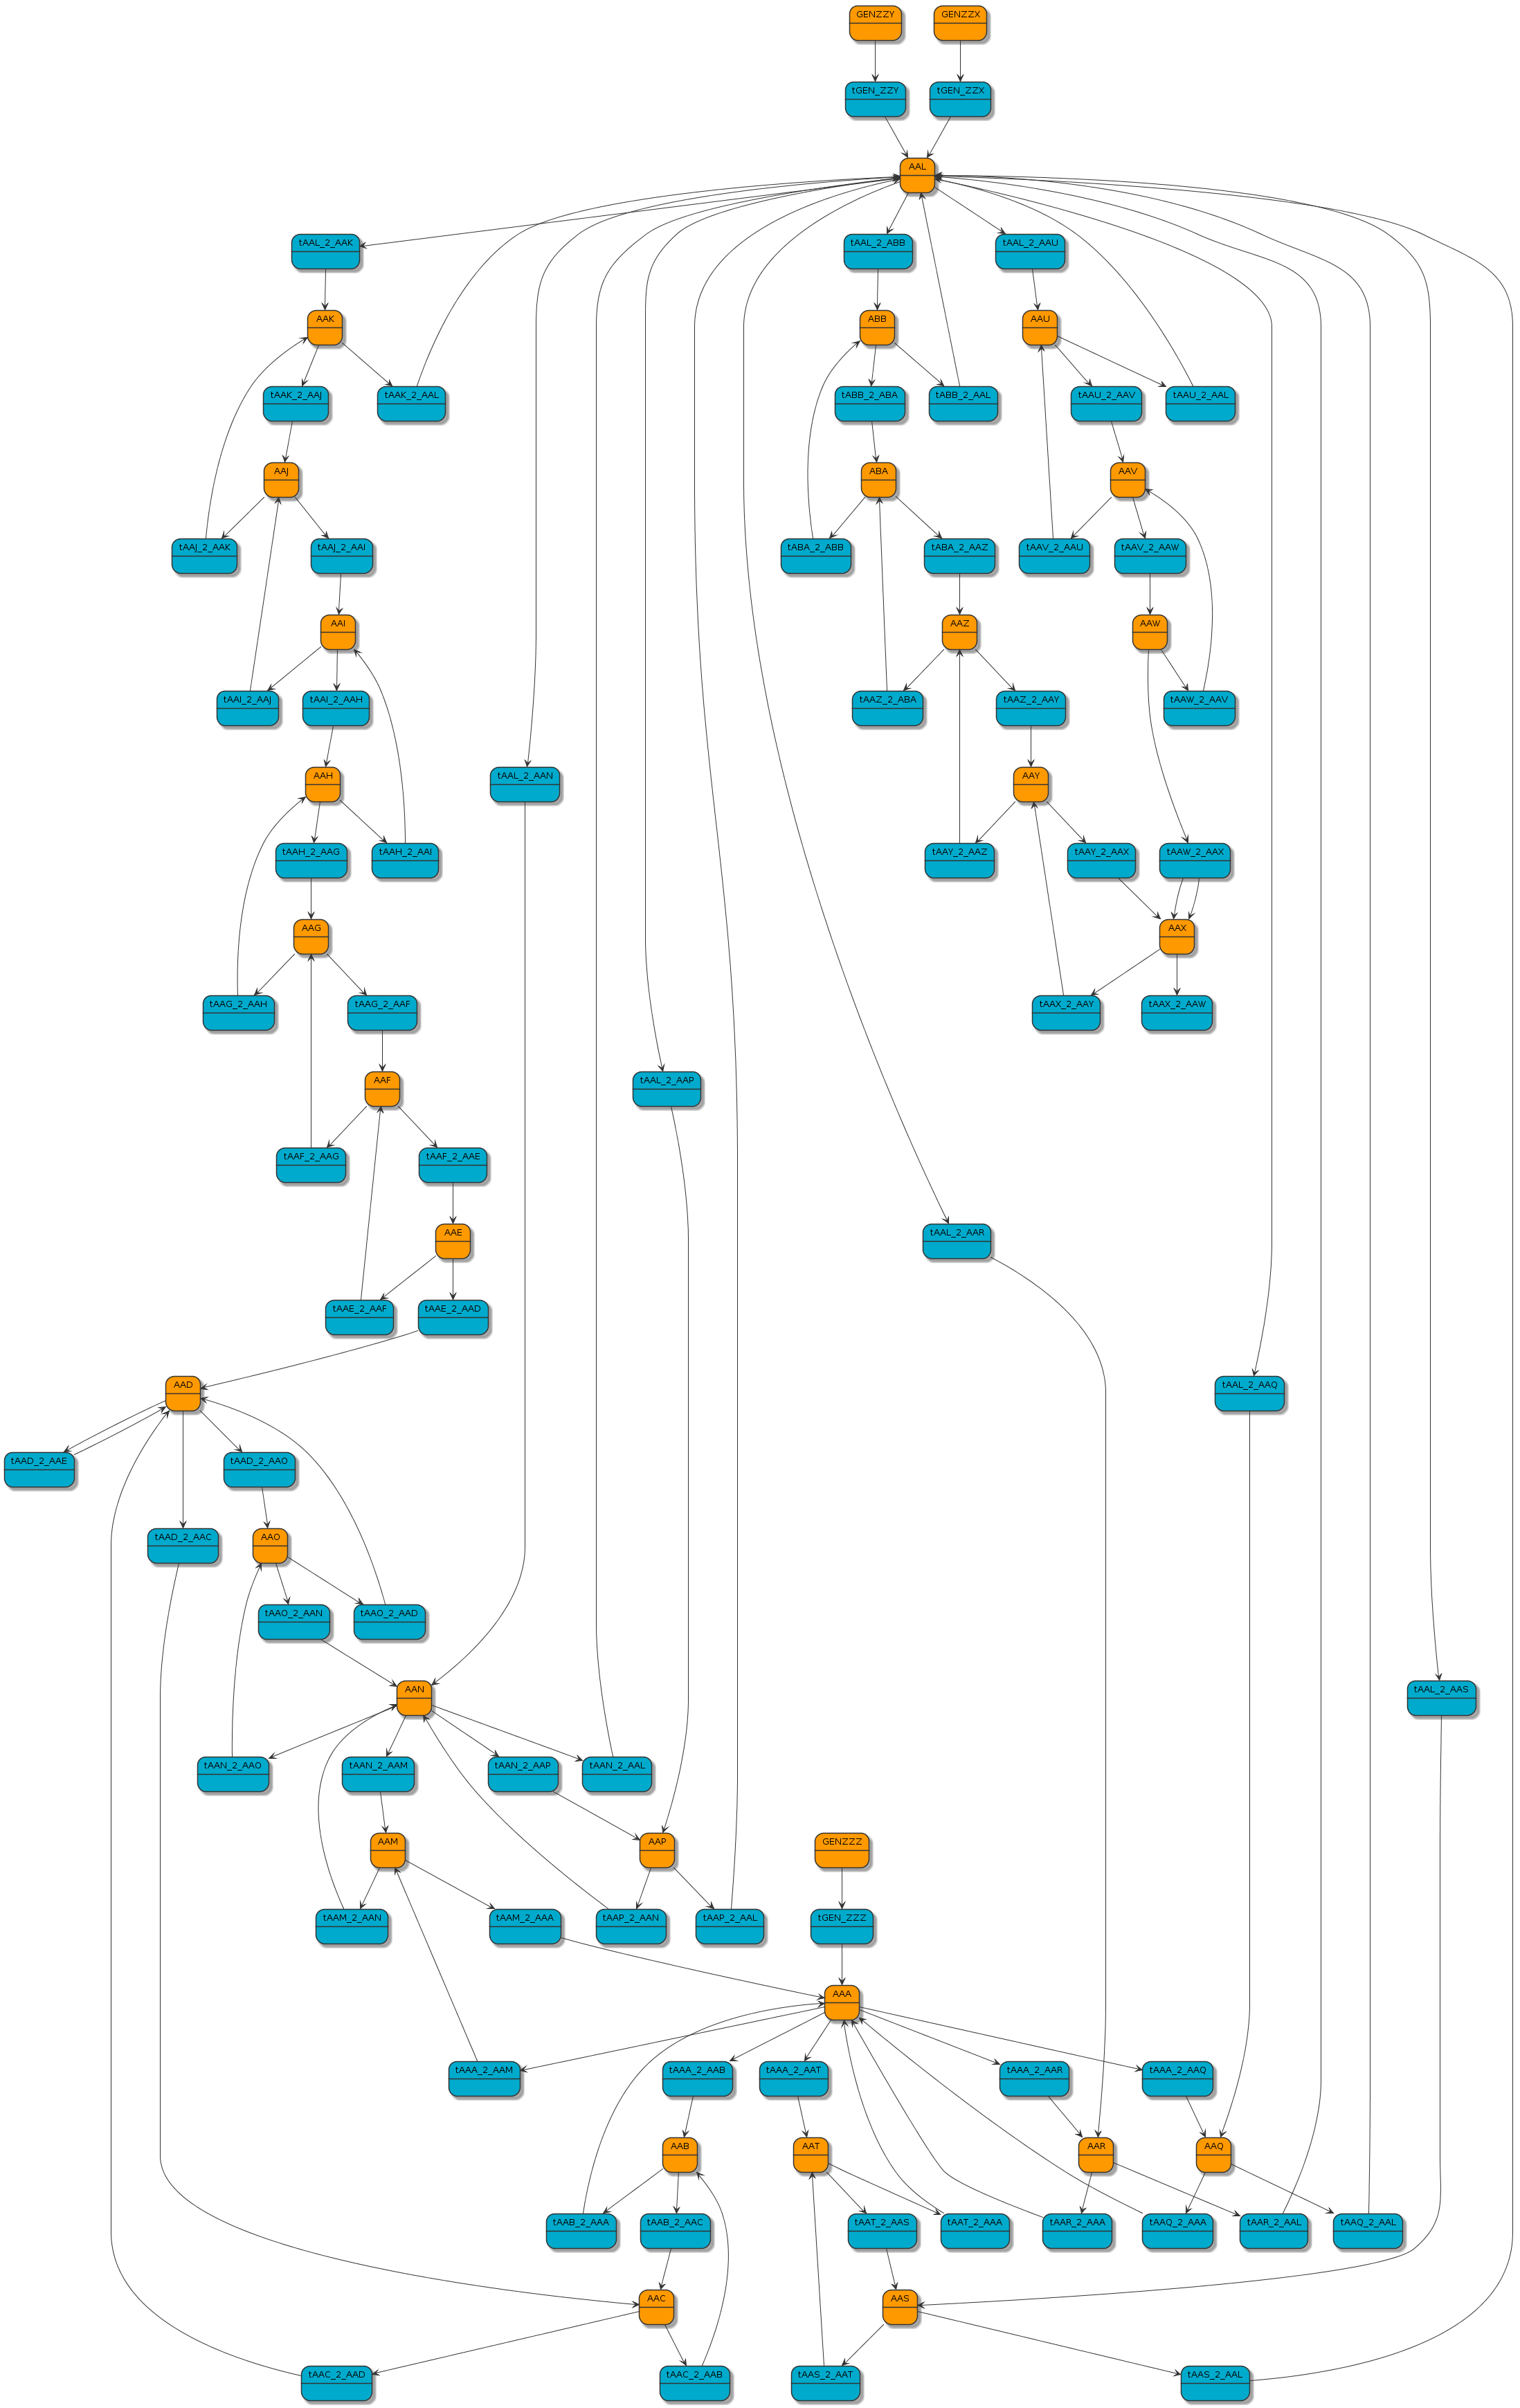
\includegraphics[scale=0.12]{schemas/img4.png}
\caption{\label{fig:img4}}
\end{figure}

\clearpage

% -------------------------------------------------------------
%
\section{Matlab approach}
\label{cha:matlabApproach}
\paragraph{}

% W pliku PDF zawarlismy definicje sieci, miejsc, przejsc i polaczen miedzy nimi. W pliku data.mat umiescilismy dane liczbowe niezbedne do przeprowadzanie symulacje. Zdecydowalismy sie na wydzielenie danych liczbowych do osobnego pliku aby poprawic czytelnosc kodu i zwiekszyc reuzywalnosc. Do powiazania danych ze soba uzylismy hasz-map ze wzgledu na latwosc wykorzystania i wzgledna efektywnosc. Dzialania wszystkich przejsc zostaly zamodelowane w pliku COMMON_PRE ze wzgledu na faktu, ze wszystkie przejscia dzialaja na tej samej zasadzie, w szczegolnosci w pliku COMMON_PRE nastepuja obliczenia zwiazane z wydluzaniem sie kabla pod wplywem badanych przez nas czynnikow oraz uwzgladnienai spadkow mocy pobieranej przez poszczeglonych odbiorcow na trasie symulacji. W [glownym pliku] zawarlismy dane niezbedne do przeorwadzenia wszystkich symulacji.

Our project consists of file containing the definition of Petri Net - places, transitions and arcs. In file data.mat we have placed numerical data which is necessary to perform simulation. We have decided to put them in single file for visibility and reusability - one can easily input new data to perform other variants of simulations. All of the transitions behaviours have been modeled in common preprocessor file because most of transitions share common behaviour. Additionally we added several functions for computing lenghtening, heating, power consumption etc.

\subsection{Main Simulation File}
\label{sec:mainSimulationFile}
\paragraph{}

Main simulation file contains loops which we used to perform a number of different simulations depending on two factors - parts of Net (routes of interest along which power is provided from generators) and external temperature (huge inpact on cable lengthening). It contains both initial set of markers distributed along generators to set which of them is active and set of priorities indicating which segment of network we are simulating.

\subsection{Loading real data}
\label{sec:loadingRealData}
\paragraph{}

To bind the data together we have used hash-maps because of their relative efficiency and ease of use. They contain values for power usage, electrical current, type of used cable, their weight. All values are bound to transition names, which afterwards are used in common preprocessor, without need to model each line separately.

\subsection{Token generator and coloring}
\label{sec:tokenGeneratorAndColoring}
\paragraph{}

Instead of use several number of tokens to simulate unit of power from generators we decided to use only one colored marker. Transition which represents one of the generators puts number of power on marker it 'generates' and later this color is being reduced with each transition, or we can say it is consumed by clients.

% -------------------------------------------------------------
%                                      
\section{Testing, analysis and results}   
\label{cha:testingAnalysisAndResults}
\paragraph{}

We have performed several simulations which have taken into consideration external temperatures ranging from -20 C to +40 C. We have also looked seperately at different parts of power grid. 


\paragraph{}
Text Text Text

% -------------------------------------------------------------
%
\section{Challenges and solutions}    
\label{cha:ChallengesAndSolutions}
\paragraph{}

The work put to this project came together with few difficulties we had to deal with.\\

Firstly, the problem itself was overly variadic and very complicated. To cope with this we had to make proper assumptions and simplifactions as described in chapter \ref{sec:assumptions}. The data we had used were taken mainly from articles we gathered and were upscaled to proper size using statistical methods. Some of the formulas used were made easier too -- for example we did omit time variable -- as it was not fit to be modeled using Petri-nets. The problem here was that the Petri-nets uses discrete variables for dealing with time tasks, while in electrical engineering the time is need to be represent as continous function.\\

Secondly, the used tool needed to store some data about the overall state of simulation in global storage. It made programming it harder and we had suffered some errors because of it.\\

Thirdly, because of naming convention and number of places and transitions it was hard to debug the whole project.\\

Last, but not least, we had to find a proper way to represent electrical power and its routing system throughout the power grid. For the first one we have chosen colors to save voltage value carried by each marker and for the second one we have used priorities. This method has been already described more in-depth in chapter \ref{cha:methods}.\\

% duzo czynnikow
% uproszczenia
% wzory
% petri-nets nie dokonaca dobrze dobrze nadaja sie do odzorowania sieci elektrycznyh
% problem z modelowaniem obustronnej komunikacji
% duzo globalnych zmiennych - zeby przechowywac dane miedzy symulacjam
% nazewnictwo
% 

% -------------------------------------------------------------
%
\section{Conclusion}
\label{cha:conclusion}
\paragraph{}

For the purpose of our project in "Modeling, simulation, and performance analysis of discrete event systems with Petri-Nets", we had simulated a part of power grid used in Poland. Our statistical analysis took into account both physical properties of cables and real topology on which power grid bases on. Using GPenSim tool \cite{Art2} we were able to model the topology of the grid into Petri-net model and then simulate its behaviour. We put focus mainly on how the cables extend and how far their temperature rises and were able to measure values of both of them. Unfortunately, the Petri-nets turned out not to be well-fit tools for this kind of task as we had initially assumed. During the project we faced many problems, but were able to solve them.\\To sum up, we believe our project was a success, we have measured everything we initially wanted despite hardships and proved things like that can be done with Petri-Nets, event if they are not perfectly convenient solution to this kind of tasks.

%W razie potrzeby projekt można w łatwy sposób rozszerzyć o uwzględnianie zmian wyżej wymienionych współczynników ze względu na elastyczność GPENSim w przeprowadzaniu obliczeń w ramach przejśc w sieci. Jednakże dane o innych wartościach parametrów nie są dostępne publicznie na stronie producentów przewodów i należałoby skontantakować się z nimi w celu uzyskaniach ich.   

% Why is this important aspect of power grid analysis? 
% Ze względu na wzrost średnich temperatur w Polsce (lub w ogólnyości na świecie) oraz stały wzrost zużycia energii elektrycznej w państawach rozwiniętych należy zwracać coraz baczniejszą uwagę na wpływ temperatur i przesyłanej mocy na stan sieci. Brak odpowiednich wyliczeń oraz prognoz może prowadzić do sytuacji w których kable zwisające na zbyt niskiej wysokości mogą prowadzić do wypadków z udziałem maszyn rolniczych lub innych pojazdów. Jest to też aspekt który każdy użytkownik może obserwować gołym okiem - np. widzimy wysoko zwisające kable w ciągu chłodnych miesięcy zimowych lub nisko podczas letnich upałów.

% Ze względu na szeroki wachlarz / szeroki zakres możliwości sieci Petriego jak i narzędzia GPENSIM model można wykorzystać zarówno do rozszerzenia dokładności symulacji wydłużania kabli jak i szeregu innych symulacji i analiz (np. strat mocy).

% -------------------------------------------------------------
%
%\listoffigures

% -------------------------------------------------------------
%
%\listoftables

% -------------------------------------------------------------
%
\clearpage
\printbibliography

%\bibliographystyle{plain}
%\bibliography{discrete-petri.bib}

%1: https://en.wikipedia.org/wiki/Thermal_expansion
%2:
%3: https://en.wikipedia.org/wiki/Petri_net}
%4: https://en.wikipedia.org/wiki/Coloured_Petri_net
%5: https://en.wikipedia.org/wiki/Thermodynamics
%6: https://pl.wikipedia.org/wiki/Rozszerzalno%C5%9B%C4%87_cieplna
%7: https://pl.wikipedia.org/wiki/Temperaturowy_wsp%C3%B3%C5%82czynnik_rezystancji
%8: https://en.wikipedia.org/wiki/Electric_power_transmission

\end{document}
